%%%%%%%%%%%%%%%%%%%%%%%%%%%%%%%%%%%%%%%%%%%%%%%%%%%%%%%%%%%%%%%%%%%%%%%%%%%%%%
% A user guide for dog stability analysis code.
%
% $Id$
%%%%%%%%%%%%%%%%%%%%%%%%%%%%%%%%%%%%%%%%%%%%%%%%%%%%%%%%%%%%%%%%%%%%%%%%%%%%%%
\documentclass[11pt,a4paper]{report}

\usepackage{
graphicx,
natbib,
bm,
amssymb,
amsmath,
amsfonts
}


\graphicspath{{./Figs/}}

\setlength{\textheight}              {245mm}
\setlength{\textwidth}               {160mm}
\setlength{\topmargin}               {-20mm}
\setlength{\oddsidemargin}           {0mm}
\setlength{\parindent}               {2.5ex}
\setlength{\leftmargin}              {2.5ex}
\setlength{\bibsep}                  {\parskip}

\renewcommand{\baselinestretch}      {1.0}
\renewcommand{\familydefault}{cmss}

\newcommand\Rey{\mbox{\textit{Re}}}
\newcommand\Str{\mbox{\textit{St}}}
\newcommand\Pra{\mbox{\textit{Pr}}}
\newcommand\Ros{\mbox{\textit{Ro}}}
\newcommand\real{{\mbox{Re}}}
\newcommand\imag{{\mbox{Im}}}
\newcommand\cd{\mathrm{d}}
\newcommand\ce{\mathrm{e}}
\newcommand\cg{\mathrm{g}}
\newcommand\ci{\mathrm{i}}
\newcommand\half{\frac{1}{2}}
\newcommand\thalf{{\textstyle{\half}}}
\newcommand\ol[1]{\overline{#1}}
\newcommand\wh[1]{\widehat{#1}}
\newcommand\wt[1]{\widetilde{#1}}
\newcommand\ob[1]{\overbrace{#1}}
\newcommand\ub[1]{\underbrace{#1}}
\newcommand\Uinf{U_\infty}
\newcommand\Vinf{V_\infty}
\newcommand\Vrel{V_\textrm{rel}}

\newcommand\NavSto{Navier--Stokes}
\newcommand\LNS{linearized \NavSto}
\newcommand\LNSE{\LNS\ equations}
\newcommand\KH{Kelvin--Helmholtz}
\newcommand\Pois{Poiseuille}
\newcommand\Orrsom{Orr--Sommerfeld}
\newcommand\GL{Ginzberg--Landau}
\newcommand\bfs{back\-ward-fac\-ing step}

\newcommand\qp{qua\-si-per\-io\-dic}
\newcommand\cc{complex-conjugate}
\newcommand\oned{one-di\-men\-sion\-al}
\newcommand\twod{two-di\-men\-sion\-al}
\newcommand\threed{three-di\-men\-sion\-al}
\newcommand\twoc{two-com\-po\-nent}
\newcommand\threec{three-com\-po\-nent}
\newcommand\gll{Gauss--Lobatto--Legendre}
\newcommand\SLO{shear-layer oscillation}
\newcommand{\ie}{i.e.\ }
\newcommand{\eg}{e.g.\ }
\newcommand\etal{{\it et al}.}

\newcommand\Ubase{{\bm{U}}}
\newcommand\Pbase{P}

\newcommand\upert{{\bm{u}'}}
\newcommand\ppert{{p}'}

\newcommand\umode{\tilde{\bm{u}}}
\newcommand\pmode{\tilde{p}}

\newcommand\xvec{\bm{x}}
\newcommand\uvec{\bm{u}}
\newcommand\uadj{\bm{u}^*}
\newcommand\qvec{\bm{q}}
\newcommand\qadj{\bm{q}^*}
\newcommand\padj{p^*}

\newcommand\qcs{\tilde{\bm{q}}}
\newcommand\qacs{\tilde{\bm{q}^*}}
\newcommand\qh{\hat{\bm{q}}}
\newcommand\qah{\hat{\bm{q}^*}}

\newcommand\Aop{{\cal A}}
\newcommand\Aadj{{\cal A^*}}
\newcommand\Hop{{\cal H}}
\newcommand\Hadj{{\cal H^*}}
\newcommand\Lop{{\cal L}}
\newcommand\Ladj{{\cal L^*}}
\newcommand\Mop{{\cal M}}
\newcommand\Madj{{\cal M^*}}

\newcommand\DN{\text{DN}}
\newcommand\DNadj{\text{DN}^*}

\newcommand\opt{\textrm{max}}
\newcommand\tauopt{\tau_\opt}
\newcommand\Gmax{G_\opt}

\hyphenation{axi-sym-met-ric}

\newcommand{\Semtex}{\emph{Semtex}}
\newcommand{\Dog}{\emph{Dog}}
\newcommand\undertext[1]{\underline{\smash{\hbox{#1}}}}

%%%%%%%%%%%%%%%%%%%%%%%%%%%%%%%%%%%%%%%%%%%%%%%%%%%%%%%%%%%%%%%%%%%%%%%%%%%%%%
\begin{document}

\begin{titlepage}
\centering

\vspace*{\fill}

{\huge Working \Dog}

\vspace{\fill}

\begin{figure}[h]
\begin{center}
\fbox{
\includegraphics[width=0.5\textwidth]{F7585}}
\end{center}
\end{figure}

\vspace{\fill}

{\large H.\,M. Blackburn}\\
Monash University

\vspace{\fill}

\today

\Dog\ version 2.0

\vspace*{\fill}

\end{titlepage}

%%%%%%%%%%%%%%%%%%%%%%%%%%%%%%%%%%%%%%%%%%%%%%%%%%%%%%%%%%%%%%%%%%%%%%%%%%%%%%

\tableofcontents

\clearpage

%%%%%%%%%%%%%%%%%%%%%%%%%%%%%%%%%%%%%%%%%%%%%%%%%%%%%%%%%%%%%%%%%%%%%%%%%%%%%
\chapter{Introduction}

\Dog\ is a tool to compute solutions to stability analysis and/or
optimal transient growth problems in steady or time-periodic viscous
flows with moderate \twod\ geometric complexity.  The name is an
acronym of '\undertext{d}irect \undertext{o}ptimal
\undertext{g}rowth'.
%
In effect \Dog\ provides an iterative eigensystem solution wrapper
around routines which timestep the linearised \NavSto\ equations and
their adjoint.

\Dog\ is built on top of the author's \Semtex\ DNS application, and so
employs quadrilateral nodal spectral elements as the underlying
discretization. It is highly recommended that you have some
familiarity with setting up and running problems in \Semtex\ before
attempting to use \Dog. If you are planning to compile \Dog\ you need
to have a working \Semtex\ installation first\,---\,please see the
setup instructions in the \Semtex\ user guide.  The default location
for the \Dog\ directory is at the same level as where you put the
\Semtex\ directory, though it is also straightforward to install it
within the \Semtex\ directory (edit \verb+dog/Makefile+).

I would very much like to acknowledge the contributions made to this
code, as well as to the ideas in the present document, by Dwight
Barkley (who originally wrote the \texttt{flok} program which was the
prototype for \Dog\ and who, together with Spencer Sherwin, helped
develop the optimal growth tools in \Dog), Ron Henderson (whose DNS
code \texttt{prism} was the underlying basis for \texttt{flok} and
which was also the progenitor of \Semtex), Spencer Sherwin and Xuerui
Mao.  It's been a great experience to work with all of you.

%=============================================================================
\section{\Dog\ and its kin}

These are the codes that can be built with the upper-level Makefile:
\begin{tabbing}
\texttt{symmetrisexx} \= \kill
% 
\texttt{dog} 
\> The central eigensystem code. Computes linear stability analysis or 
optimal \\
\> transient growth for a two-dimensional base flow.\\
%
\texttt{lns} 
\> Integrate the linearised \NavSto\ equations and/or their adjoint\\ 
\> (\eg to evolve an eigenmode or optimal initial condition).\\ 
\> This drives exactly the same routines that \texttt{dog} uses.\\
%
\texttt{normalize} 
\> Normalise an eigenmode or initial condition \\
\> (\eg so it has unit kinetic energy per unit mass).\\
%
\texttt{combine} 
\> Combine a base flow with an eigenmode/IC to
produce an initial condition \\ \> \emph{in physical space} (\eg for
subsequent evolution using \texttt{dns}, part of \Semtex).\\
%
\texttt{circulate} 
\> `Rotate' a sequence of base flows to generate a different starting phase\\ 
\> for Floquet or transient analysis.\\
%
\texttt{flipmap} 
\> Generate a set of mapping indices for a `half-period flip'.\\
%
\texttt{symmetrise} 
\> Enforce a reflection symmetry (from flipmap) on a field file.
\end{tabbing}

There are also a couple of more specialised executables that can be
built: \texttt{dog-H} \citep[for computing stability with a
  half-period flip, see e.g.][]{bml05} and \texttt{dog-AR} which uses
\texttt{ARPACK} \citep{lehoucq98} as the Arnoldi eigensystem solver as
opposed to the (default) `Barkley' method documented in
\citet{bbs08b}.

%============================================================================
\subsection{Files}

Just like \Semtex, \Dog\ needs a starting input file which describes
the mesh, boundary conditions, and sets up tokens used by the solver.
We call this a \verb+session+ file and typically it has no root
extension.  It is written in a format patterned on HTML, which we
have called FEML (for Finite Element Markup Language). An extra input
file required by \Dog\ is \verb+session.bse+ which contains the base
flow. There are a number of example session files in the mesh
directory.  Other files have standard extensions:
\begin{tabbing}
\texttt{session.bsexxxx} \= \kill 
%
\texttt{session.bse}  \>
        Base flow on which analysis is performed.  Same format as
        \texttt{session.fld}.\\
\texttt{session.evl} \> Eigenvalue (and convergence) information.\\
\texttt{session.eig.X} \> Eigenvector \texttt{X}. 
     Same format as \texttt{session.fld}\\
\texttt{session.fld}  \>
        Solution/field file.  Binary format by default.\\
\texttt{session.num}  \>
        Global node numbers, produced by enumerate utility.\\
\texttt{session.rst}  \>
        Restart file. Read in to initialize solution if present.\\
\texttt{session.avg} \> Averaged results. Read back in for
        continuation (over-written).\\
\texttt{session.his} \> History point data.\\
\texttt{session.mdl} \> Time series of kinetic energies in the Fourier
        modes (only for 3D execution).\\
\end{tabbing}
The primary focus when running \Dog\ is usually the \verb+session.evl+
file. It is good practice to use \verb+tail -f session.evl+ in order
to monitor progress of convergence.


%============================================================================
\subsection{Usage}


%%%%%%%%%%%%%%%%%%%%%%%%%%%%%%%%%%%%%%%%%%%%%%%%%%%%%%%%%%%%%%%%%%%%%%%%%%%%%%
\chapter{Theory}
\label{ch.theory}

Two good general references for the methods advanced in this chapter
are \citet{tuba00} and \citet{bbs08b}.

%=============================================================================
\section{The \LNSE\ in operator form}

We start with the incompressible \NavSto\ equations
\begin{equation}
\partial_t\uvec=-\uvec\bm{\cdot \nabla}\uvec -\bm{\nabla} p
+\Rey^{-1}\nabla^2 \uvec, \quad \text{with} \quad\bm{\nabla\cdot}\uvec=0,
\end{equation}
where $p$ is the modified or kinematic pressure, $\uvec$ is the
velocity vector, while the Reynolds number $\Rey=UD/\nu$ where $U$ and
$D$ are convenient velocity and length scales and $\nu$ is kinematic
viscosity. 
%
Decomposing the flow field as the sum of a base flow and a
perturbation \ie $(\uvec,p)=(\Ubase,P)+(\upert,\ppert)$ we first substitute
\begin{equation}
\partial_t(\Ubase+\upert) = -(\Ubase+\upert)\bm{\cdot\nabla}(\Ubase+\upert)
  - \bm{\nabla}(\Pbase+\ppert)
  + \Rey^{-1}\nabla^2(\Ubase+\upert),
\end{equation}
expand
\begin{equation}
\partial_t(\Ubase+\upert) =
-\Ubase\bm{\cdot\nabla}\Ubase
-\Ubase\bm{\cdot\nabla}\upert
-\upert\bm{\cdot\nabla}\Ubase
-\upert\bm{\cdot\nabla}\upert
- \bm{\nabla}(\Pbase+\ppert)  
+ \Rey^{-1}\nabla^2(\Ubase+\upert), 
\end{equation}
then collect into equations for evolution of the base flow
\begin{equation}
\partial_t\Ubase =
-\Ubase\bm{\cdot\nabla}\Ubase
- \bm{\nabla}\Pbase
+ \Rey^{-1}\nabla^2\Ubase,
\end{equation}
and perturbation
\begin{equation}
\partial_t\upert =
-\Ubase\bm{\cdot\nabla}\upert
-\upert\bm{\cdot\nabla}\Ubase
-\upert\bm{\cdot\nabla}\upert
- \bm{\nabla}\ppert
+ \Rey^{-1}\nabla^2\upert,
\end{equation}
from which we omit interaction of perturbations (assuming those terms
to be $O(\upert^2)$), to obtain the \LNSE, which
govern the evolution of infinitesimal perturbations, as
\begin{equation}
\partial_t\upert
=-[\bm{U \cdot\nabla}+(\bm{\nabla U})^T\bm{\cdot}] \upert 
-\bm{\nabla} \ppert+\Rey^{-1}\nabla^2 \upert.
\label{eqn.LNS} 				
\end{equation}

We note that the base flow $\Ubase$ does not have to be steady in
time: it may also be time-periodic, or have more general structure.

Considering that in incompressible flow the pressure may be considered
a constraint field whose gradient keeps the flow divergence-free and
which is obtained from the advection terms as the solution of a
Poisson equation, we can say that
\begin{equation}
\ppert\equiv
\nabla^{-2}\bm{\nabla\cdot}\left[\Ubase\bm{\cdot\nabla}
+(\bm{\nabla\Ubase})^\text{T}\bm{\cdot}\right]\upert
\end{equation}
and so we can write the \LNS\ symbolically without the pressure term as
\begin{equation}
\partial_t\upert =
-\left[\bm{I}-\bm{\nabla}\nabla^{-2}\bm{\nabla\cdot}\right]
\left[\Ubase\bm{\cdot\nabla}
  +(\bm{\nabla\Ubase})^\text{T}\bm{\cdot}\right]\upert
+ \Rey^{-1}\nabla^2\upert,
\end{equation}
or more compactly, since now the spatial terms are now just a linear
operator applied to the perturbation velocity, we write the
\LNS\ equations in operator form as
\begin{equation}
\partial_t\upert-\Lop(\upert)=0.		
\label{eq.lns}
\end{equation}
The above notation is adopted largely for compactness/convenience and
does not imply that the pressure is not computed.  However, it is
typically only the velocity components which are considered as part of
the numerical eigensystem analysis of incompressible flows.

%=============================================================================
\section{Timestepping, the exponential mapping, and eigensystems}

So now let us consider the effect of evolving (time-integrating,
timestepping) a perturbation $\upert$ from an initial state at (let's
say) $t=0$ over a time interval (period, horizon) $\tau$.
\begin{equation}
\upert_\tau=\Mop(\tau)\upert_0
\label{eq.STO}
\end{equation}
where 
\begin{equation}
\Mop(\tau) = \exp \int_{t=0}^{t=\tau}\Lop(t)\,\cd t
\end{equation}
is the state transition operator of the \LNSE. We note
that \eqref{eq.STO} is symbolic shorthand for `apply the
\LNS\ equations to an initial condition by time-integration over
interval $\tau$' and is what we approximate when running a simulation
code that evolves our numerical approximation to the \LNSE.  It is
also important to note that in carrying out this numerical integration
the time interval $\tau$ is typically broken into a large number of
time steps $\Delta t$.
%

%-----------------------------------------------------------------------------
\subsection{Linear stability analysis of steady flows}

If $\Ubase$ is steady in time, then so is $\Lop$, in which case $\Mop$
has a particularly simple written form
\begin{equation}
\Mop(\tau)=\exp(\Lop\tau).
\label{eq.map}
\end{equation}

We now turn to the problem of finding the eigensystems of $\Lop$ or
equivalently of $\Mop(\tau)$.  Recall that the eigensystem of $\Lop$
is the set of eigenvalues $\lambda_j$ and eigenvectors (or `mode
shapes') $\wt{\bm{u}}_j(\xvec)$ which satisfy
\begin{equation}
\Lop \wt{\bm{u}}_j = \lambda_j \wt{\bm{u}}_j.
\label{eq.eig}
\end{equation}
Staying for now with the case that $\Ubase$ is steady in time, the
large-time asymptotic behaviour of solutions to the \LNSE\ is
determined by the eigensystem of operator $\Lop$ written in terms of
its eigenvalues and eigenvectors
\begin{equation}
\upert(\xvec, t) = \sum_{j=0}^\infty
\exp(\lambda_j t)\wt{\bm{u}}_j(\xvec) +\text{c.c.}
\label{eq.sep}
\end{equation}
where we will consider that the eigenvalues may be complex
($\lambda=\omega_r\pm\ci\omega_i$) but the eigenvectors are real. The
set of all the eigenvalues of an operator is called its spectrum. We
note that (as is sometimes reversed in textbooks) $\omega_r$ is a
growth rate and $\omega_i$ is a (circular) frequency.  We also note
that \eqref{eq.eig} is generated directly by substituting the
separation-of-variables form \eqref{eq.sep} into \eqref{eq.lns}. A
linear stability analysis of a \NavSto\ problem amounts to finding the
leading (least stable) eigenvalues of $\Lop$ and the corresponding
mode shapes (perturbation flows).  This gives the large-time behaviour
of linear perturbations\,---\,we will deal with the finite-time
behaviour later.

Now, for simple flows (\eg \oned\ base flows), we may be able to
afford to explicitly construct a matrix approximation for the operator
$\Lop$ and find its full eigensystem directly \citep[see \eg appendix
  A of][]{schmid01}. However, for more complicated flows a direct
solution may be very expensive computationally (in both time and
memory) and we typically have to resort to iterative methods.
Iterative eigensystem solvers of the Arnoldi type \citep{saad92} rely
on repeatedly applying an operator (matrix) to a vector, as in
\eqref{eq.STO}, without necessarily explicitly contructing the
operator itself. Such methods are typically best at converging those
eigenpairs which have eigenvalues of largest magnitude, \ie the part
of the spectrum furthest from the origin in the complex plane.  Also,
for stability problems we are usually mostly concerned with the
eigenvalues $\lambda_j$ with largest real part (\ie the least stable
eigenvalues) and do not much care about more stable modes. By happy
coincidence the exponential mapping \eqref{eq.map} has precisely the
feature of transforming the spectrum in such a way that the
least-stable eigenvalues of $\Lop$ become the largest-magnitude
eigenvalues of $\Mop$, as indicated in figure~\ref{fig.map}.  This
means that timestepper-based methods for evolving the \LNSE\ are very
well matched to iterative methods for finding (the leading part of)
the eigensystem of an operator.

\begin{figure}
\begin{center}
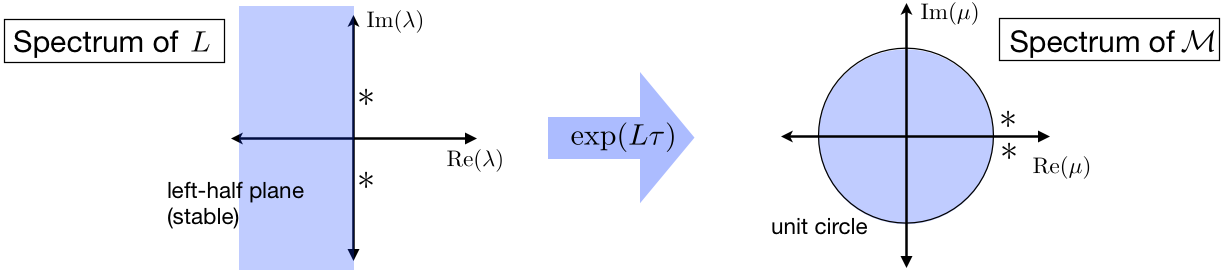
\includegraphics[width=\textwidth]{mapping}
\end{center}
\caption{The timestepper mapping. Left left-half plane of $\Lop$ is
  mapped to inside the unit circle of $\Mop$, and there is a
  one-to-one mapping of the spectrum of the two operators.}
\label{fig.map}
\end{figure}

The eigensystems of $\Lop$ and $\Mop$ are connected.  Since
\begin{equation}
\exp \Lop\tau =
\lim_{N\to\infty}
\sum_{k=0}^{N}
\frac{\left(\Lop\tau\right)^k}{k!}
\end{equation}
we find that the eigenvectors of $\Lop$ are the same as those of
$\Mop(\tau)$: supposing $\wt{\bm{u}}_j$ is an eigenvector of $\Lop$ with
corresponding eigenvalue $\lambda_j$.  Then
\begin{equation}
\Mop\wt{\bm{u}}_j=
\exp \Lop\tau\,\wt{\bm{u}}_j=
\lim_{N\to\infty}\sum_{k=0}^N\frac{\left(\Lop\tau\right)^k}{k!}\wt{\bm{u}}_j=
\lim_{N\to\infty}\sum_{k=0}^N\frac{\left(\lambda_j \tau\right)^k}{k!}\wt{\bm{u}}_j=
\exp(\lambda_j\tau)\wt{\bm{u}}_j,
\end{equation}
\ie $\wt{\bm{u}}_j$ is also an eigenvector of $\Mop(\tau)$, with
corresponding mapped eigenvalue $\mu_j=\exp(\lambda_j\tau)$.  In fact,
since we will be finding the (complex) eigenvalues
$\mu_j=\sigma_{r,j}\pm\ci\sigma_{i,j}$ of $\Mop(\tau)$, we note that
their polar magnitudes and angles in the complex plane are given by
\begin{equation}
|\mu_j|=(\sigma_{r,j}^2+\sigma_{i,j}^2)^{1/2},\qquad
\angle\mu_j=\pm\arctan(\sigma_{i,j}/\sigma_{r,j})
\end{equation}
(using the `two-argument' $\arctan$ function).  From these values we
can work back to find the real and imaginary parts of the eigenvalues
$\lambda_j$ of $\Lop$:
\begin{equation}
\omega_{r,j}=\ln(|\mu_j|)/\tau,\qquad
\omega_{i,j}=(\angle\mu_j)/\tau.
\end{equation}

The base flow is (linearly) neutrally stable when the largest
$|u_j|=1$ or equivalently when the least stable mode has
$\omega_{r,j}=0$.  Finding the parameter(s) which results in neutral
stability is usually the primary focus of a flow stability
analysis. This value is typically referred to as the `critical' value,
\eg critical Reynolds number.

%-----------------------------------------------------------------------------
\subsection{Linear stability analysis of time-periodic flows}

If $\Ubase$ is time-periodic, then so is the operator $\Lop$ and we
carry out temporal Floquet stability analysis \citep[analysis of a
  linear system of ODEs/PDEs where the coefficients are time-periodic,
  see e.g.][]{iooss90}. In this case, we are typically interested in
how much a disturbance grows from one period of the base flow to the
next.  The method of analysis is in fact very similar to that
described above for steady base flows, but now the time integration
period $\tau$ is fixed to match the period of the base flow, and the
eigenmodes are also time-dependent (and time-periodic).  In this case
\begin{equation}
\upert(\xvec, t+\tau) = \sum_{j=0}^\infty
\mu_j\wt{\bm{u}}_j(\xvec,t\,\textrm{mod}\,\tau) +\text{c.c.}
\label{eq.flok}
\end{equation}
Note the general similarity to \eqref{eq.sep}, but that the
eigenvectors (or Floquet modes) are now time-periodic.  The
eigenvalues $\mu_j$ are referred to a Floquet multipliers.  Since the
analysis now has a distinct `digital' aspect (performed on a
$\tau$-periodic basis) it now only really makes much sense to consider
dealing directly with the timestepper mapping \eqref{eq.STO} and only
be concerned with the right side of figure~\ref{fig.map}.  The Floquet
multipliers say how much a mode grows or shrinks over a period: if
they lie outside the unit circle, the mode grows; if inside, it
shrinks.  A good general reference on global Floquet analysis is the
classic paper by \citet{bah96}.  If the multiplier $\mu=-1$, the
instability is of period-doubling or subharmonic type; if it has
non-zero imaginary part (occurs in complex conjugate pairs) the
instability is \qp\ \citep{bllo03b}.

The base flow for Floquet analysis is usually provided as a set of
time-slices equispaced over $\tau$, and Fourier reconstruction is the
typical means of re-estimating the base flow at any point in its
period.  We note that if the base flow has features which are very
sharp in time (as observable in velocity time-history plots), a
considerable number of time-slices may be needed for accurate
reconstruction, and then Fourier reconstruction may become very
costly; in this case a local cubic spline reconstruction may be used
instead, since the interpolation cost is lower \citep{msb11}.
%
(It is also possible to carry along computation of the base flow as a
separate operation in parallel, an approach sometimes adopted in other
codes.)

As mentioned above, the Floquet modes are time-periodic, although the
multiplier associated with each mode is a fixed scalar.  A single
Floquet analysis generally only returns the mode (or modes, if more
than one is requested) at one particular phase, the starting phase of
the base flow. If one requires the modes at another phase point, one
can either rotate the order of the base flows (using \Dog's
\verb+circulate+ utility), or ask for a time-shift (as a command-line
argument to \verb+dog+).

%==============================================================================
\section{Optimal growth of perturbations}

The motivation for understanding optimal non-normal growth of
perturbations is that if linear non-normal growth is large enough,
non-linear mechanisms may take over and produce a transition to
turbulence even if the flow is linearly stable in the long term
\citep[see e.g.][]{srk02}.
%
The standard introductory text of this area is \citet{schmid01}.

Since the \LNSE\ are non-symmetric (the operator written in on a
comp\-on\-ent-by-component matrix form is non-symmetric about the
leading diagonal), its eigenmodes are in general `non-normal', meaning
that the energy inner products of distinct modes may be non-zero (\ie
the modes are non-orthogonal or non-normal).  This is different from,
say, the eigenmodes of a spring--mass system, which does have this
property, leading to the ability to examine energetics on a
mode-by-mode basis which is a considerable simplification.  

In order to examine these issues and to consider the growth of
perturbations, we need to introduce energy-type integrals.
%
Flow is considered within a spatial domain $\Omega$ which has a
boundary surface $\partial\Omega$ and unit outward normal $\bm{n}$, as
indicated in figure~\ref{fig.domain}.  Flow is taken to evolve over
the time interval $[0,\tau]$, so the space-time domain considered is
$\Omega\times[0,\tau]$.

\begin{figure}
\begin{center}
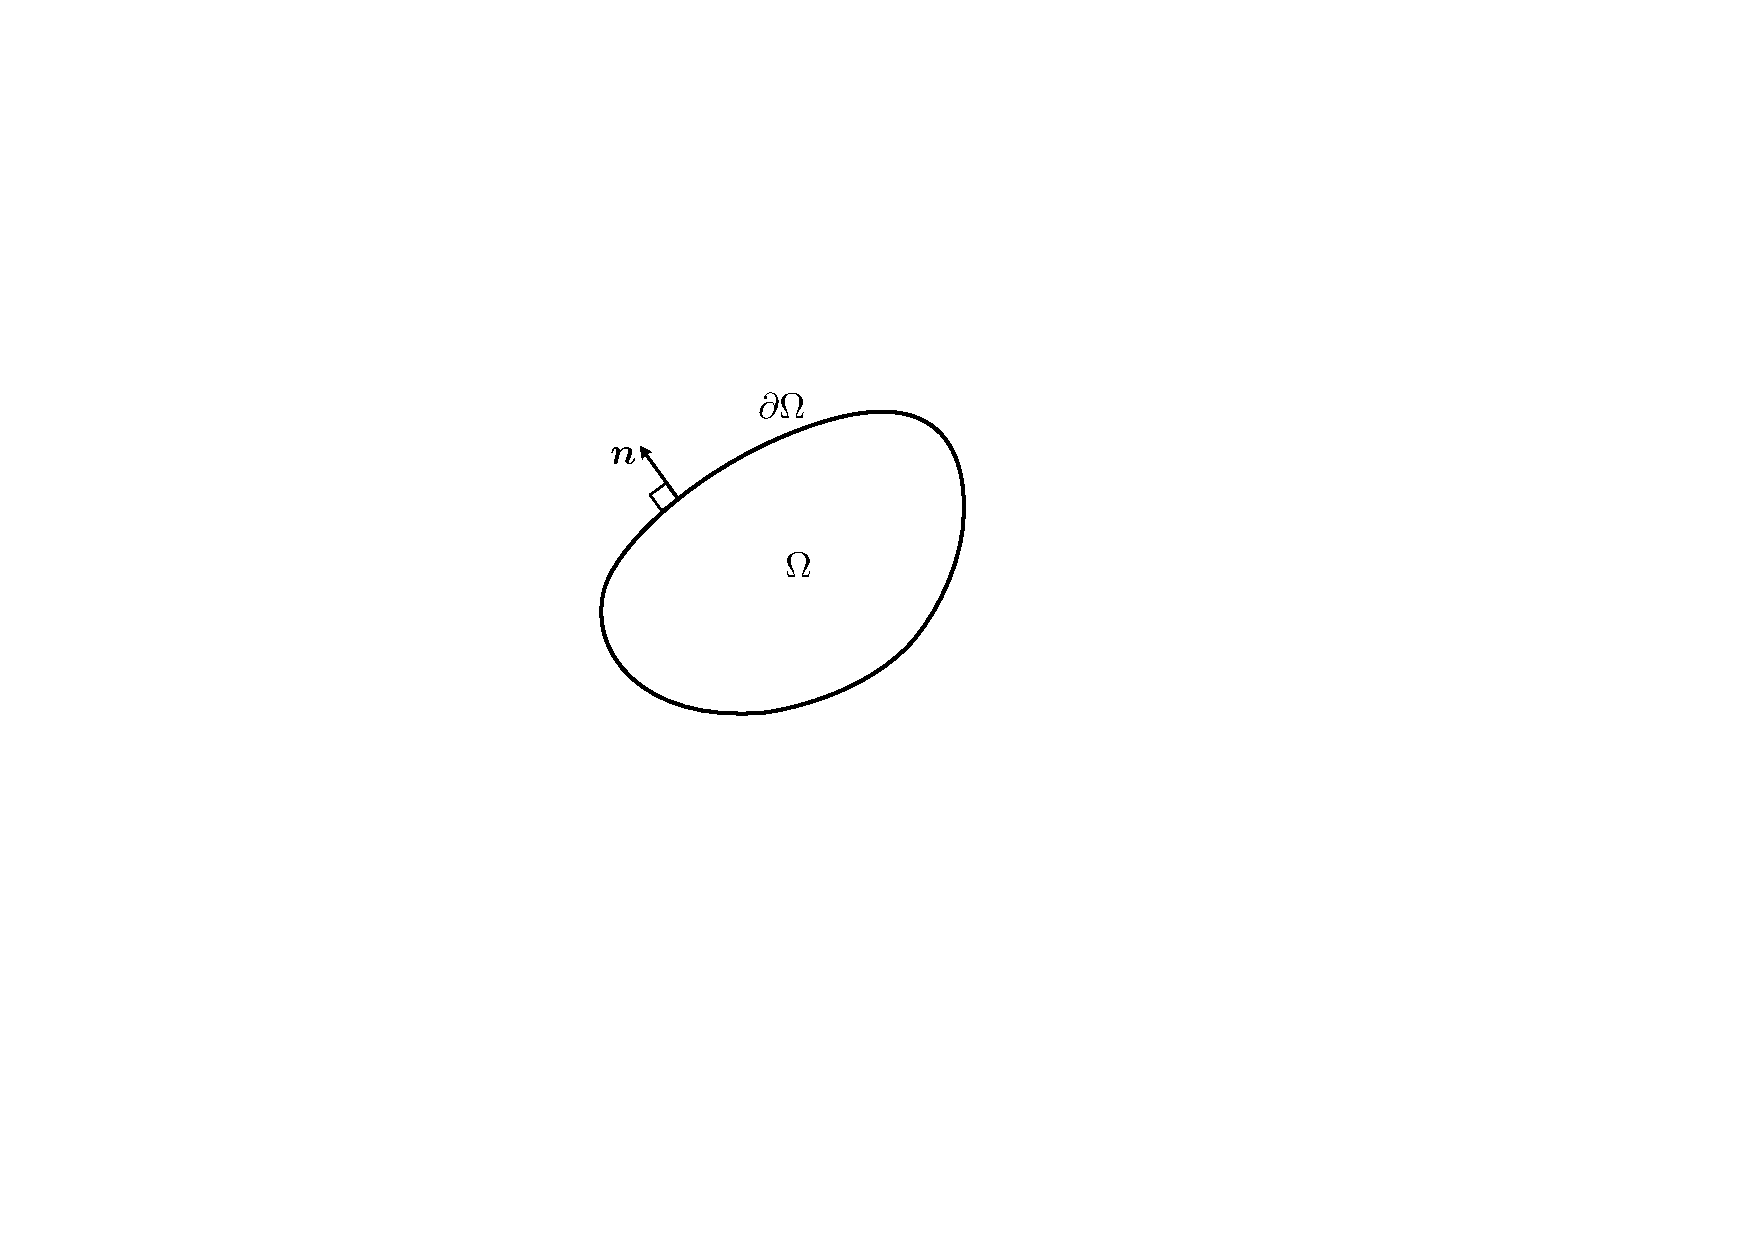
\includegraphics[width=0.25\textwidth]{generaldomain}
\end{center}
\caption{Schematic representation of a spatial flow domain $\Omega$,
  boundary $\partial\Omega$ and unit outward normal vector $\bm{n}$.}
\label{fig.domain}
\end{figure}

The energy inner product of two modes on domain $\Omega$ can be
written as
\begin{equation}
E=(\wt{\bm{u}}_i, \wt{\bm{u}}_j) = \int_\Omega \wt{\bm{u}}_i
  (\xvec)\bm{\cdot} \wt{\bm{u}}_j^\ast(\xvec)\,\cd V,
\end{equation}
where the superscript $\ast$ denotes complex conjugate.  If the modes
are orthogonal (and suitably normalised) then $(\wt{\bm{u}}_i,
\wt{\bm{u}}_j)=\delta_{i,j}$ where $\delta_{i,j}$ is the Kronecker
delta, in which case
\begin{align}
\nonumber
(\upert,\upert)(t)&=
\int_\Omega\left(\sum_{i=1}^N\exp(\lambda_i t)
\wt{\uvec}_i\right)\bm{\cdot}
\left(\sum_{j=1}^N\exp(\lambda_j^\ast t)\wt{\uvec}_j^\ast\right)\,\cd V\\
\nonumber
& =\sum_{i=1}^N\sum_{j=1}^N
\exp(\lambda_i t)\exp(\lambda_j^\ast t)
\int_\Omega\wt{\uvec}_i\bm{\cdot}\wt{\uvec}_j^\ast\,\cd V\\
&=\sum_{i=1}^N\exp(2\,\text{Re}(\lambda_i)\, t),
\end{align}
leading to the result that if all modes are stable then the kinetic
energy of a linear perturbation has to decay exponentially in time.
If the modes are non-normal, then this property is lost and energy of
a linear perturbation composed of stable modes may grow in the short
term, perhaps very considerably, before eventual decay.
\citet{schmid01} give a particularly simple geometric illustration of
how this can occur in their figure~4.1, reproduced here as
figure~\ref{fig.tg}.

\begin{figure}
\begin{center}
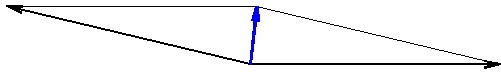
\includegraphics[width=0.3\textwidth]{nn0000.png}\\
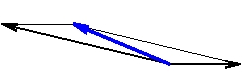
\includegraphics[width=0.3\textwidth]{nn0025.png}\\

\includegraphics[width=0.3\textwidth]{nn0040.png}\\

\includegraphics[width=0.3\textwidth]{nn0070.png}\\

\includegraphics[width=0.3\textwidth]{nn0080.png}\\

\includegraphics[width=0.3\textwidth]{nn0100.png}
\end{center}
\caption{Transient growth resulting from the sum (blue) of two
  non-orthogonal eigenvectors (black), each of which decays.  Adapted
  from figure~4.1, \cite{schmid01}. The asymptotic state is decay
  dominated by the least stable eigenvector. }
\label{fig.tg}
\end{figure}

Now consider energy growth $G$, \ie the ratio of kinetic energies in a
linear disturbance at time $t=\tau$ to that in the initial condition
at time $t=0$.
\begin{equation}
G(\tau)=\frac{E(\tau)}{E(0)}=
\frac{(\bm{u}'_\tau,\bm{u}'_\tau)}{(\bm{u}'_0,\bm{u}'_0)}=
\frac{(\Mop(\tau)\bm{u}'_0,\Mop(\tau)\bm{u}'_0)}{(\bm{u}'_0,\bm{u}'_0)},
\end{equation}
where the last equality exploits \eqref{eq.STO}.  Our goal is to find
the `most dangerous', or optimal, initial disturbance $\uvec'_0$; the
one that generates the greatest amount of growth $G$ for time interval
$\tau$.  Various routes exist for the computation of such an optimum
\citep{mbs13}; here we will examine the `eigenvalue approach'.

%%%%%%%%%%%%%%%%%%%%%%%%%%%%%%%%%%%%%%%%%%%%%%%%%%%%%%%%%%%%%%%%%%%%%%%%%%%%%%
\chapter{Stability analysis of steady flows}

It is assumed that you already have some familiarity with \Semtex.
The DNS tool from \Semtex, \texttt{dns}, is typically (though as you
will find out in the first example, not always) used to generate the
base flows on which analysis is performed.


%=============================================================================
\section{Two-dimensional stability of Poiseuille channel flow}

The two-dimensional parabolic-profile flow in a parallel channel
becomes linearly unstable to Tollmein--Schlichting waves at
$\Rey=5772$ \citep{ors71}.  For $\Rey=7500$ and at streamwise
wavenumber $\alpha=1$ (\ie a wavelength of $2\pi$) based on the
semi-channel width, \citet[\S\,1.4]{chqz88} supply estimates of the
eigenvalue $\omega=0.00223497+\ci 0.24989154$ (the temporal growth
rate is the first of these values and the second is the temporal
circular frequency).  This is a rather simple problem because the
domain is rectangular, the base flow is analytic, and also the
eigenmode is 2D2C\,---\,\twod\ and \twoc.  (While a global stability
analysis is overkill for this problem, it certainly is
straightforward.)

First, we'll make a session file. Since the domain is rectangular, we
can use the \Semtex\ \verb+rectmesh+ utility, which makes a startup
session file that we can edit to create a workable session file for
our problem.  Below is the rectmesh input file (made with a text
editor) that we'll call \verb+channel.rect+.  The format is: list of
$x$-locations; blank line; list of $y$-locations.  Don't worry that
the length is $\Delta x=2$ rather than $2\pi$; we will fix that by
editing the session file that we produce.

{\small
\begin{verbatim}
-1
-0.75
-0.5
-0.25
0
0.25
0.5
0.75
1

-1
-0.8
-0.5
0
0.5
0.8
1
\end{verbatim}
}

Next we create our session file:
{\small
\begin{verbatim}
[mec-aquila]$ rectmesh channel.rect > channel
\end{verbatim}
}

Edit the resulting session file to produce:
{\small
\begin{verbatim}
<TOKENS>
        X_SCALE  = PI

        N_SLICE  = 1
        N_BASE   = 2

        N_TIME   = 2
        N_P      = 11
        N_STEP   = 200
        D_T      = 0.005
        Re_D     = 7500
        KINVIS   = 1/Re_D

        IO_HIS   = 20
        IO_FLD   = 1000
        IO_CFL   = 20
</TOKENS>

<FIELDS NUMBER=3>
        u      v       p
</FIELDS>

<GROUPS NUMBER=1>
        1       w       wall
</GROUPS>

<BCS NUMBER=1>
        1       w       3
                <D>     u = 0.0  </D>
                <D>     v = 0.0  </D>
                <H>     p        </H>
</BCS>

<USER>
        u = 1-y*y
        v = 0.
        p = 0.
</USER>

<NODES NUMBER=63>
    1	             -1             -1              0
    2	          -0.75             -1              0
    ..
    ,,
    ..
    62	           0.75              1              0
    63	              1              1              0
</NODES>

<ELEMENTS NUMBER=48>
    1	<Q>    1    2   11   10    </Q>
    2	<Q>    2    3   12   11    </Q>
    ..
    ..
    ,,
    47	<Q>   52   53   62   61    </Q>
    48	<Q>   53   54   63   62    </Q>
</ELEMENTS>

<SURFACES NUMBER=22>
         1   1  1  <B>  w  </B>
         2   2  1  <B>  w  </B>
         3   3  1  <B>  w  </B>
         4   4  1  <B>  w  </B>
         5   5 	1  <B>  w  </B>
         6   6  1  <B>  w  </B>
         7   7  1  <B>  w  </B>
         8   8  1  <B>  w  </B>

         9  41  3  <B>  w  </B>
        10  42  3  <B>  w  </B>
        11  43  3  <B>  w  </B>
        12  44  3  <B>  w  </B>
        13  45  3  <B>  w  </B>
        14  46  3  <B>  w  </B>
        15  47  3  <B>  w  </B>
        16  48  3  <B>  w  </B>

        17   8  2  <P>   1  4  </P>
        18  16  2  <P>   9  4  </P>
        19  24  2  <P>  17  4  </P>
        20  32  2  <P>  25  4  </P>
        21  40  2  <P>  33  4  </P>
        22  48  2  <P>  41  4  </P>
</SURFACES>
\end{verbatim}
}
\noindent
(Note that various repetitious lines have been deleted from the above
listing.)

%-----------------------------------------------------------------------------
\subsection{\texttt{TOKENS} section}

Let us first examine the \verb+TOKENS+ used.  Setting
\verb+X_SCALE=PI+ is used to expand the overall length of the domain
to $2\pi$ (this scaling is not specific to \Dog, but is a normal part
of \Semtex).  
%
The next two tokens are, however, specific to \Dog: \verb+N_SLICE=1+
says that there will be only a single time-slice in the base flow file
(the base flow is steady in time), while \verb+N_BASE=2+ stipulates
that the base flow should only have two velocity components ($x$ and
$y$ components $u$ and $v$).
%
Setting \verb+N_TIME=2+ stipulates 2nd-order accurate time stepping
(this could be omitted since it is the default value, but you may
occasionally want to use \verb+N_TIME=1+ or
\verb+N_TIME=3+). \verb+N_P=11+ will give 11 mesh points along the
side of each quadrilateral element so that the element shape functions
will be tensor products of 10th-order GLL-Lagrange interpolants.
%
\verb+N_STEP=200+ and \verb+D_T=0.005+ together mean that the
time-step is $\Delta t=0.005$ and 200 steps are taken for each
integration of the linearised \NavSto\ equations over an interval
$\delta t=1$ between Arnoldi updates.  Both these values (time step
and interval between updates) ultimately need to be chosen on the
basis of trial and error\,---\,at least, that is the case for a steady
flow stability analysis: for a time-periodic base flow the interval is
pre-determined and only the time-step needs to be set.
%
\verb+Re_D=7500+ and \verb+KINVIS=1/Re_D+ are used to set the
kinematic viscosity: we could have directly set
\verb+KINVIS=0.0001333333333+ but here we see the built-in function
parser used to set the value (token \verb+Re_D+ is not otherwise
significant to the solver).

%-----------------------------------------------------------------------------
\subsection{\texttt{FIELDS} section}

This is used to tell the solver that 3 fields will be be used and they
are two velocity components $u$ and $v$ along with pressure $p$.  NB:
the pressure is not normally considered to be part of the eigensystem
and further that the pressure variable contained in the
\verb+session.eigX+ file is normally unreliable (BUT one can force it
to be included using the \verb+-p+ command-line option to
\verb+dog+). Also note that the \verb+NUMBER+ of fields must be
specified in the section header (this is not required in normal
\Semtex\ usage).

%-----------------------------------------------------------------------------
\subsection{\texttt{GROUPS} and \texttt{BCS} sections}

Standard \Semtex\ usage. Read that user guide!

%-----------------------------------------------------------------------------
\subsection{\texttt{USER} section}

While again this is standard \Semtex\ usage, we note that in the
present case we will be using this section along with the standard
utility \texttt{compare} in order to generate our base flow.  Again
observe the implied use of the built-in function parser to deal with
the string \verb+u = 1-y*y+ and that coordinate \verb+y+ (along with
\verb+x+ and \verb+t+) is known to the parser.

%-----------------------------------------------------------------------------
\subsection{\texttt{NODES}, \texttt{ELEMENTS} and \texttt{SURFACES} sections}

Standard \Semtex.  However, note the use of \verb+<P>+ in the
\verb+SURFACES+ section to declare periodic edges.

%-----------------------------------------------------------------------------
\subsection{Base flow generation}

Normally we would have to use \texttt{dns} to generate a steady base
flow (typically by integrating to reach the asymptotically steady
state, a task which might well reqire its own session file and time
stepping).  In the present case, though, have an analytic base flow
declared in our session file and can use the \verb+compare+ utility to
parse the strings in the \verb+USER+ section.
{\small
\begin{verbatim}
[mec-aquila]$ compare channel > channel.bse
\end{verbatim}
} This creates a base flow with $u=1-y^2$, $v=0$ and $p=0$ (the
pressure is not used and could in fact be omitted).

%-----------------------------------------------------------------------------
\subsection{Make an enumeration file}

We have retained standard \Semtex\ requirement that a
\verb+session.num+ file must be produced. If not explicitly created,
one will be generated on the fly, but it is usually better to make one
`by hand' in order to ensure that the highest-level RCM numbering
optimisation level (3) is obtained.
{\small
\begin{verbatim}
[mec-aquila]$ enumerate -O3 channel > channel.num
\end{verbatim}
}


%-----------------------------------------------------------------------------
\subsection{Running \texttt{dog}}

Now we are ready. I'll assume commands from \Dog\ (like all the
\Semtex\ commands we've used to this point) will be found in your
\texttt{PATH}.
{\small
\begin{verbatim}
[mec-aquila]$ dog -k 16 -n 1 -m 500 -t 1e-6 channel > /dev/null &
\end{verbatim}
}The command line arguments above have the following sigificance:
\verb+-k 16+, set the Krylov dimension to 16; \verb+-n 1+, stop after
one eigenvalue is convereged to the requested tolerance;
\verb+-m 500+, iterate for a mximum of 500 iterations; \verb+-t 1e-6+,
carry on converging until the residual for the higest-numbered
eigenvalue requested (here just one) falls below this tolerance value
(multiplied by the growth magnitude.

The first time you run \verb+dog+ you might not want to suppress the
standard output as we have done here in order to ensure everything is
running correctly. However, the usage above is generally standard
since it alllows the user to monitor convergence of the eigensystem
solver by running tail on the \verb+session.evl+ file.  {\small
\begin{verbatim}
[mec-aquila]$ tail -f -18 channel.evl
\end{verbatim}
} This will show us updates to the end of the eigenvalue file.  After
a number of iterations the solution terminates with {\small
\begin{verbatim}
-- Iteration = 265, H(k+1, k) = 0.894358
EV  Magnitude   Angle       Growth      Frequency   Residual
 0  1.0022e+00  2.4989e-01  2.2358e-03  2.4989e-01  9.7943e-07
 1  1.0022e+00 -2.4989e-01  2.2358e-03 -2.4989e-01  9.7943e-07
 2  9.6002e-01  9.5902e-01 -4.0801e-02  9.5902e-01  1.6653e-03
 3  9.6002e-01 -9.5902e-01 -4.0801e-02 -9.5902e-01  1.6653e-03
 4  9.9859e-01  0.0000e+00 -1.4078e-03  0.0000e+00  5.2856e-03
 5  9.9644e-01  0.0000e+00 -3.5696e-03  0.0000e+00  1.4456e-02
 6  9.4387e-01  1.9403e+00 -5.7764e-02  1.9403e+00  3.7580e-02
 7  9.4387e-01 -1.9403e+00 -5.7764e-02 -1.9403e+00  3.7580e-02
 8  9.8493e-01  0.0000e+00 -1.5188e-02  0.0000e+00  4.1501e-02
 9  9.2051e-01  2.9086e+00 -8.2826e-02  2.9086e+00  2.3085e-01
10  9.2051e-01 -2.9086e+00 -8.2826e-02 -2.9086e+00  2.3085e-01
11  8.9517e-01  1.6337e+00 -1.1075e-01  1.6337e+00  3.5807e-01
12  8.9517e-01 -1.6337e+00 -1.1075e-01 -1.6337e+00  3.5807e-01
13  7.6534e-01  2.2901e+00 -2.6743e-01  2.2901e+00  7.4006e-01
14  7.6534e-01 -2.2901e+00 -2.6743e-01 -2.2901e+00  7.4006e-01
15  2.8354e-01  3.1416e+00 -1.2604e+00  3.1416e+00  8.3424e-01
dog: converged, writing 1 eigenvectors.
\end{verbatim}
} You should find that file \verb+channel.eig.0+ now exists: this is
the leading eigenvector (not written out unless convergence is
obtained): we only get one because only one was requested
(\verb+-n 1+).  In fact since the leading eigenvalue is complex, we
could have converged both the leading eigenvector and its `complex
conjugate' which in this case will be real-valued, just like the
 leading eigenvector, but phase-shifted a quarter-period in time, \ie
 translated along the channel. We will return to that point below.

Let us examine the significance of the listing above.  The first point
is that 265 iterations were required for convergence, largely
reflecting the fact that there is not a great deal of separation of
the magnitudes of the leading eigenvalues, as an inspection of the
less-converged values indicates.



%%%%%%%%%%%%%%%%%%%%%%%%%%%%%%%%%%%%%%%%%%%%%%%%%%%%%%%%%%%%%%%%%%%%%%%%%%%%%%
\chapter{Stability analysis of time-periodic flows}


%%%%%%%%%%%%%%%%%%%%%%%%%%%%%%%%%%%%%%%%%%%%%%%%%%%%%%%%%%%%%%%%%%%%%%%%%%%%%%
\chapter{Optimal growth analysis}



%%%%%%%%%%%%%%%%%%%%%%%%%%%%%%%%%%%%%%%%%%%%%%%%%%%%%%%%%%%%%%%%%%%%%%%%%%%%%

\bibliographystyle{dcu}
\bibliography{userguide}

%%%%%%%%%%%%%%%%%%%%%%%%%%%%%%%%%%%%%%%%%%%%%%%%%%%%%%%%%%%%%%%%%%%%%%%%%%%%%
\end{document}
